\documentclass[14pt]{beamer}

\usepackage{tikz}
\usetikzlibrary{arrows,fit,backgrounds}
\usetikzlibrary{positioning}
\usepackage[noend]{algpseudocode}
\algtext*{EndIf}

\tikzset{arrowin/.style={<-,>=latex,semithick},arrowout/.style={->,>=latex,semithick},root/.style={circle,draw,line width=2pt},box/.style={rectangle, rounded corners, minimum width=1cm, minimum height=1cm,text centered, draw=black}}
\tikzstyle{arrowin}=[<-,>=latex,semithick]
\tikzstyle{arrowout}=[->,>=latex,semithick]
\tikzstyle{root}=[circle,draw,line width=2pt]

\usepackage{epstopdf}
\usepackage{xcolor}

\renewcommand{\arraystretch}{1.5}
\newcommand{\tuple}[1]{\ensuremath{\left \langle #1 \right \rangle }}

\usetheme{Madrid}
\usecolortheme{dolphin}
\setbeamertemplate{footline}{} % removes the entire footline
\setbeamertemplate{navigation symbols}{} % removes navigation symbols that would appear on the bottom right of each slide.
\setbeamertemplate{enumerate items}[default] % enumerates with standard numbers instead of graphics.
\setbeamertemplate{blocks}[rounded]
\setbeamertemplate{bibliography item}[text]


\setbeamertemplate{headline}
{
\begin{beamercolorbox}[ht=6ex,dp=2ex,center]{title in head/foot}
\usebeamerfont{subtitle}\insertsection
\end{beamercolorbox}
}

\addtobeamertemplate{title page}{
\includegraphics[scale=0.5]{logo.eps}}{}
\title{\textbf{A Reference Interpreter for the Graph Programming Language GP 2}}
\author{Christopher Bak$^1$, Glyn Faulkner$^1$, Colin Runciman and Detlef Plump}
\institute{Department of Computer Science, The University of York}
\date[GaM 2015]{Graphs as Models, April 2015\\[1em]
{\scriptsize $^1$Supported by EPRSC Doctoral Training Grants.}}

\begin{document}

\begin{frame}
  \titlepage
\end{frame}

\begin{frame}{Outline}
\begin{itemize}\setlength{\itemsep}{10mm}
\item The GP 2 Language
\item The GP 2 Reference Interpreter
\item Conclusions and Future Work
\end{itemize}
\end{frame}

\section{GP 2}

\begin{frame}{Graph Programs}
\begin{itemize}
\item Domain-specific language for graph-based structures.
\item User supplies the input graph and the graph transformation rules.
\item Small imperative language to organise rule applications.
\item Non-deterministic execution.
\item Simple syntax and semantics to facilitate formal reasoning.
\end{itemize}
\end{frame}

\begin{frame}{Structured Operational Semantics}
\begin{center}
\begin{tabular}{lcl}
$\mathrm{[Call_1]} \displaystyle\frac{G \Rightarrow_{R} H}{\langle R,G\rangle \to H}$ 
&&
$\mathrm{[Call_2]} \displaystyle\frac{G \nRightarrow_{R}}{\langle R,G\rangle \to \texttt{fail}}$ 
\\\\
$\mathrm{[Alap_1]} \displaystyle\frac{\langle P, G\rangle \to^+ H}{\langle P!, G\rangle \to \langle P!, H\rangle}$ 
&&
$\mathrm{[Alap_2]} \displaystyle\frac{\langle P, G\rangle \to^+ \texttt{fail}}{\langle P!, G\rangle \to G}$ 
\\\\
\end{tabular} 
\end{center}
\begin{itemize}
\item The states are graphs (G and H) and \texttt{fail}.
\item R is a rule. P is a program.
\end{itemize}
\end{frame}

\begin{frame}{Transitive Closure}
\begin{center}
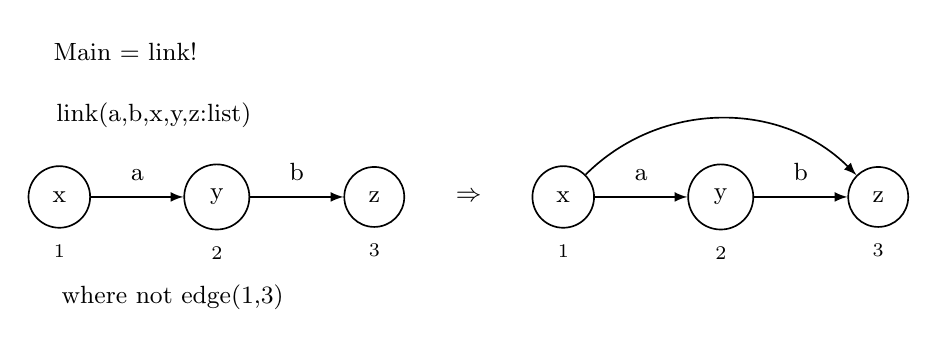
\begin{tikzpicture} [scale=0.8,align=center,auto,inner sep=2mm,arrowin,arrowout,font=\ttfamily]

\tikzstyle{every text node part}=[font=\small]

\node at (1.05,2.3) {Main = link!};
\node at (1.5,1.3) {link(a,b,x,y,z:list)};

\node (l1) at (0,0)[circle,draw,label=below:\scriptsize{1}]{x};
\node (l2) at (2.5,0)[circle,draw,label=below:\scriptsize{2}]{y}
  edge [<-] node[above]{a} (l1);
\node (l3) at (5,0)[circle,draw,label=below:\scriptsize{3}]{z}
  edge [<-] node[above]{b} (l2);

\node at (6.5,0){$\Rightarrow$};

\node (r1) at (8,0)[circle,draw,label=below:\scriptsize{1}]{x};
\node (r2) at (10.5,0)[circle,draw,label=below:\scriptsize{2}]{y}
  edge [<-] node[above]{a} (r1);
\node (r3) at (13,0)[circle,draw,label=below:\scriptsize{3}]{z}
  edge [<-] node[above]{b} (r2)
  edge [<-, bend right=45] (r1);

\node at (1.8,-1.6) {where not edge(1,3)};
\end{tikzpicture}

\end{center}
\begin{itemize}
\item Rule \texttt{link} applied as long as possible on the input graph.
\item List labels used for generality.
\end{itemize}
\end{frame}

\begin{frame}{Vertex Colouring}
\begin{center}
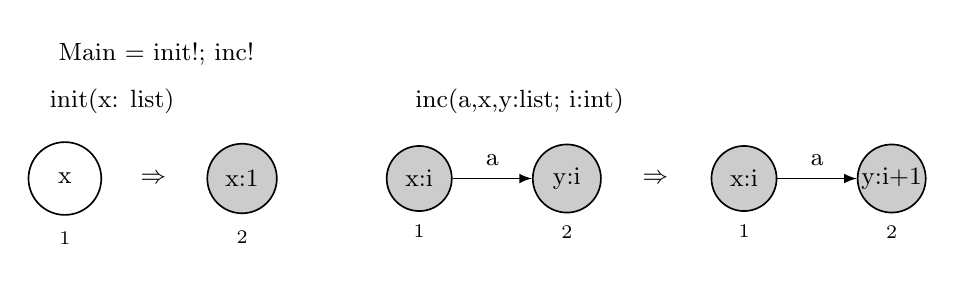
\begin{tikzpicture} [scale=0.75,align=center,auto,inner sep=2mm,arrowin,arrowout,font=\ttfamily]

\tikzstyle{every text node part}=[font=\small]

\node at (1.55,2.1) {Main = init!; inc!};
\node at (0.8,1.3) {init(x: list)};
\node at (0,0)[circle,draw,inner sep=2.5mm,label=below:\scriptsize{1}]{x};
\node at (1.5,0){$\Rightarrow$};
\node at (3,0)[circle,draw,inner sep=1.5mm,fill=black!20,label=below:\scriptsize{2}]{x:1};

\begin{scope}[inner sep=1.5mm,xshift=6cm]
\node at (1.7,1.3) {inc(a,x,y:list; i:int)};

\node (l1) at (0,0)[circle,draw,fill=black!20,label=below:\scriptsize{1}]{x:i};
\node (l2) at (2.5,0)[circle,draw,fill=black!20,label=below:\scriptsize{2}]{y:i}
  edge [<-] node[above]{a} (l1);

\node at (4,0){$\Rightarrow$};

\node (r1) at (5.5,0)[circle,draw,fill=black!20,label=below:\scriptsize{1}]{x:i};
\node (r2) at (8,0)[circle,draw,inner sep=0.2mm,fill=black!20,label=below:\scriptsize{2}]{y:i+1}
  edge [<-] node[above]{a} (r1);
\end{scope}

\end{tikzpicture}

\end{center}
\begin{itemize}
\item Always outputs a valid colouring.
\item Minimal colouring not guaranteed because of non-determinism.
\end{itemize}
\end{frame}

\begin{frame}{Vertex Colouring}
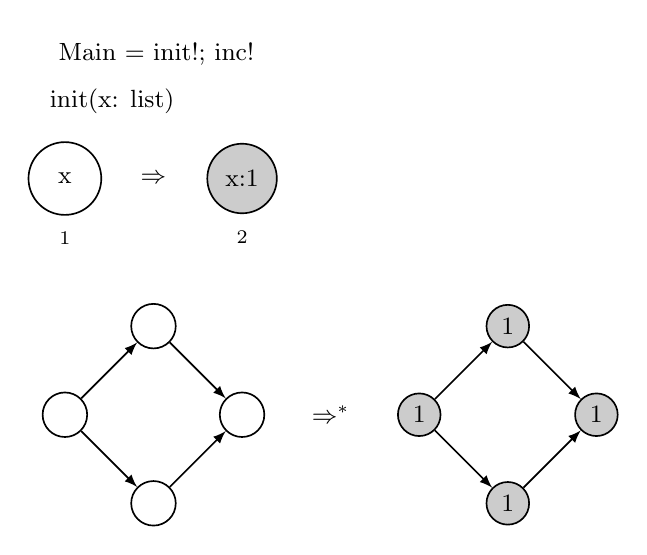
\begin{tikzpicture} [scale=0.75,align=center,auto,inner sep=2mm,arrowin,arrowout,font=\ttfamily]

\tikzstyle{every text node part}=[font=\small]

\node at (1.55,2.1) {Main = init!; inc!};
\node at (0.8,1.3) {init(x: list)};
\node at (0,0)[circle,draw,inner sep=2.5mm,label=below:\scriptsize{1}]{x};
\node at (1.5,0){$\Rightarrow$};
\node at (3,0)[circle,draw,inner sep=1.5mm,fill=black!20,label=below:\scriptsize{2}]{x:1};

\begin{scope}[yshift=-4cm]
\node (g1) at (0,0)[circle,draw]{};
\node (g2) at (1.5,1.5)[circle,draw]{}
  edge[<-] (g1);
\node (g3) at (1.5,-1.5)[circle,draw]{}
  edge[<-] (g1);
\node (g4) at (3,0)[circle,draw]{}
  edge[<-] (g2)
  edge[<-] (g3);

\node<2> at (4.5,0){$\Rightarrow^*$};

\node<2> (g1) at (6,0)[circle,draw,inner sep=1mm,fill=black!20]{1};
\node<2> (g2) at (7.5,1.5)[circle,draw,inner sep=1mm,fill=black!20]{1}
  edge[<-] (g1);
\node<2> (g3) at (7.5,-1.5)[circle,draw,inner sep=1mm,fill=black!20]{1}
  edge[<-] (g1);
\node<2> (g4) at (9,0)[circle,draw,inner sep=1mm,fill=black!20]{1}
  edge[<-] (g2)
  edge[<-] (g3);
\end{scope}

\end{tikzpicture}

\end{frame}

\begin{frame}{Vertex Colouring}
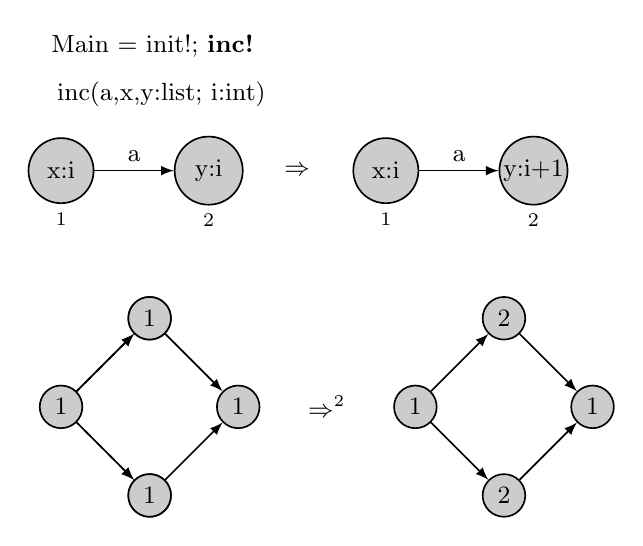
\begin{tikzpicture} [scale=0.75,align=center,auto,inner sep=1mm,arrowin,arrowout,font=\ttfamily]

\tikzstyle{every text node part}=[font=\small]

\node at (1.55, 2.1) {Main = init!; \textbf{inc!}};
\node at (1.7,1.3) {inc(a,x,y:list; i:int)};

\node (l1) at (0,0)[circle,draw,fill=black!20,inner sep=1.5mm,label=below:\scriptsize{1}]{x:i};
\node (l2) at (2.5,0)[circle,draw,fill=black!20,inner sep=1.5mm,label=below:\scriptsize{2}]{y:i}
  edge [<-] node[above]{a} (l1);

\node at (4,0){$\Rightarrow$};

\node (r1) at (5.5,0)[circle,draw,fill=black!20,inner sep=1.5mm,label=below:\scriptsize{1}]{x:i};
\node (r2) at (8,0)[circle,draw,inner sep=0.2mm,fill=black!20,label=below:\scriptsize{2}]{y:i+1}
  edge [<-] node[above]{a} (r1);

\begin{scope}[yshift=-4cm]
\node (g1) at (0,0)[circle,draw,fill=black!20]{1};
\node<1>(g2) at (1.5,1.5)[circle,draw,fill=black!20]{1}
  edge[<-, dashed] (g1);
\node<2>(g2) at (1.5,1.5)[circle,draw,fill=black!20]{1}
  edge[<-] (g1);
\node<1>(g3) at (1.5,-1.5)[circle,draw,fill=black!20]{1}
  edge[<-, dashed] (g1);
\node<2>(g3) at (1.5,-1.5)[circle,draw,fill=black!20]{1}
  edge[<-] (g1);
\node (g4) at (3,0)[circle,draw,fill=black!20]{1}
  edge[<-] (g2)
  edge[<-] (g3);

\node<2> at (4.5,0){$\Rightarrow^2$};

\node<2> (g1) at (6,0)[circle,draw,fill=black!20]{1};
\node<2> (g2) at (7.5,1.5)[circle,draw,fill=black!20]{2}
  edge[<-] (g1);
\node<2> (g3) at (7.5,-1.5)[circle,draw,fill=black!20]{2}
  edge[<-] (g1);
\node<2> (g4) at (9,0)[circle,draw,fill=black!20]{1}
  edge[<-] (g2)
  edge[<-] (g3);
\end{scope}

\end{tikzpicture}

\end{frame}

\begin{frame}{Vertex Colouring}
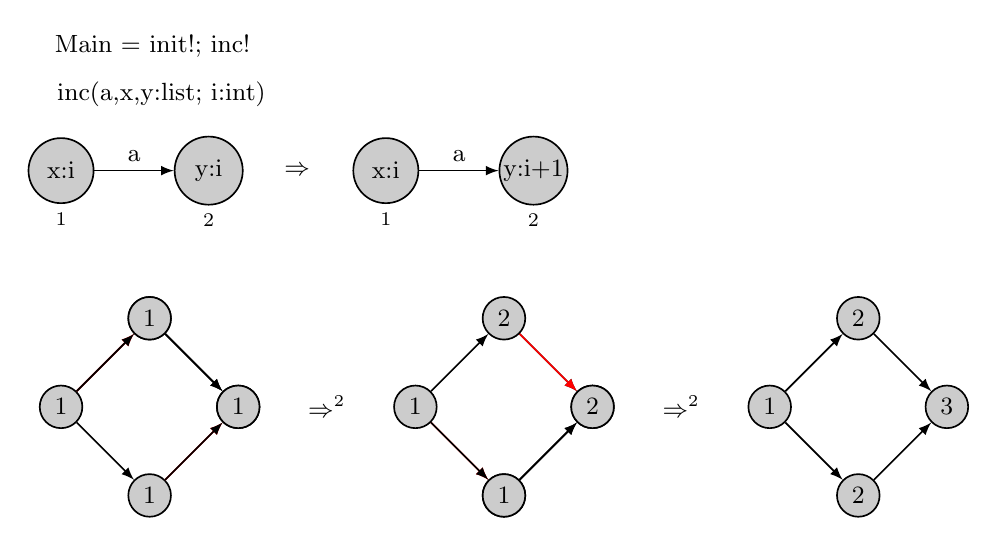
\begin{tikzpicture} [scale=0.75,align=center,auto,inner sep=1mm,arrowin,arrowout,font=\ttfamily]

\tikzstyle{every text node part}=[font=\small]

\node at (1.55, 2.1) {Main = init!; inc!};
\node at (1.7,1.3) {inc(a,x,y:list; i:int)};

\node (l1) at (0,0)[circle,draw,fill=black!20,inner sep=1.5mm,label=below:\scriptsize{1}]{x:i};
\node (l2) at (2.5,0)[circle,draw,fill=black!20,inner sep=1.5mm,label=below:\scriptsize{2}]{y:i}
  edge [<-] node[above]{a} (l1);

\node at (4,0){$\Rightarrow$};

\node (r1) at (5.5,0)[circle,draw,fill=black!20,inner sep=1.5mm,label=below:\scriptsize{1}]{x:i};
\node (r2) at (8,0)[circle,draw,inner sep=0.2mm,fill=black!20,label=below:\scriptsize{2}]{y:i+1}
  edge [<-] node[above]{a} (r1);

\begin{scope}[yshift=-4cm]
\node (g1) at (0,0)[circle,draw,fill=black!20]{1};
\node<1>(g2) at (1.5,1.5)[circle,draw,fill=black!20]{1}
  edge[<-, red] (g1);
\node<2->(g2) at (1.5,1.5)[circle,draw,fill=black!20]{1}
  edge[<-] (g1);
\node (g3) at (1.5,-1.5)[circle,draw,fill=black!20]{1}
  edge[<-] (g1);
\node<1>(g4) at (3,0)[circle,draw,fill=black!20]{1}
  edge[<-] (g2)
  edge[<-, red] (g3);
\node<2->(g4) at (3,0)[circle,draw,fill=black!20]{1}
  edge[<-] (g2)
  edge[<-] (g3);

\node<2-> at (4.5,0){$\Rightarrow^2$};

\node<2-> (g1) at (6,0)[circle,draw,fill=black!20]{1};
\node<2-> (g2) at (7.5,1.5)[circle,draw,fill=black!20]{2}
  edge[<-] (g1);
\node<2> (g3) at (7.5,-1.5)[circle,draw,fill=black!20]{1}
  edge[<-, red] (g1);
\node<3> (g3) at (7.5,-1.5)[circle,draw,fill=black!20]{1}
  edge[<-] (g1);
\node<3> (g4) at (9,0)[circle,draw,fill=black!20]{2}
  edge[<-] (g2)
  edge[<-] (g3);
\node<2> (g4) at (9,0)[circle,draw,fill=black!20]{2}
  edge[<-, red] (g2)
  edge[<-] (g3);

\node<3> at (10.5,0){$\Rightarrow^2$};

\node<3> (g1) at (12,0)[circle,draw,fill=black!20]{1};
\node<3> (g2) at (13.5,1.5)[circle,draw,fill=black!20]{2}
  edge[<-] (g1);
\node<3> (g3) at (13.5,-1.5)[circle,draw,fill=black!20]{2}
  edge[<-] (g1);
\node<3> (g4) at (15,0)[circle,draw,fill=black!20]{3}
  edge[<-] (g2)
  edge[<-] (g3);
\end{scope}

\end{tikzpicture}

\end{frame}

\begin{frame}{Motivation}

\begin{itemize}
\itemsep1pt\parskip0pt\parsep0pt
\item
  familiarise ourselves with the semantics of GP 2
\item
  identify any gaps or ambiguities in the semantics
\item
  testing correctness of later compiled implementations
\end{itemize}

\end{frame}

\begin{frame}{Requirements 1}

General requirements:

\begin{itemize}
\itemsep1pt\parskip0pt\parsep0pt
\item
  Quick to develop 
\item
  Easy to maintain and reason about
\item
  Must be fast enough to do ``useful work''
\end{itemize}

\pause

For a given program/host-graph pair\ldots{}

\begin{itemize}
\itemsep1pt\parskip0pt\parsep0pt
\item
  Produce all distinct output graphs up to isomorphism 
\item
  Generate all possible output graphs 
\item
  Output a single result 
\end{itemize}

\end{frame}

\begin{frame}{Requirements 2}

Also, stand-alone tools:

\begin{itemize}
\itemsep1pt\parskip0pt\parsep0pt
\item
  isomorphism checker
\item
  graph viewer (based on GraphViz)
\end{itemize}

\end{frame}

\begin{frame}{Implementation 1}

\begin{itemize}
\itemsep1pt\parskip0pt\parsep0pt
\item
  Written in Haskell\footnote{\url{https://www.haskell.org/}}
\item
  As close as possible to a direct translation of the GP 2 semantics
\end{itemize}

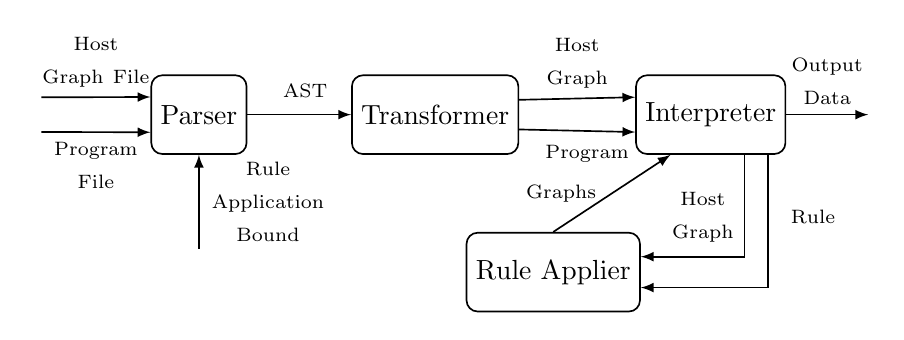
\begin{tikzpicture} [align=center, arrowout]

\node(parser) at (0,0)  [box, rounded corners] {Parser};

\node(gen) at (3,0) [box, rounded corners] {Transformer};

\node(inter) at (6.5,0) [box, rounded corners] {Interpreter};

\node(apply) at (4.5,-2) [box, rounded corners] {Rule Applier};

\draw[arrowout] (-2, 0.22) -- node[above, text width=1.5cm]{\scriptsize{Host Graph File}} (parser.160);
\draw[arrowout] (-2, -0.22) -- node[below, text width=1.5cm]{\scriptsize{Program File}} (parser.200);
\draw[arrowout] (0,-1.7) -- node[right, text width=1.5cm]{\scriptsize{Rule Application Bound}} (parser.270);

\draw [arrowout] (parser) --  (gen);
\node at (1.35,0.3) {\scriptsize{AST}};

\draw [arrowout] (gen.10) -- node[above, text width=1cm]{\scriptsize{Host Graph}} (inter.167);
\draw [arrowout] (gen.350) --  (inter.193);
\node at (4.9,-0.5) [text width=1cm]{\scriptsize{Program}};

\draw [arrowout] (inter.325) |- (apply.350);
\node at (7.8,-1.3) {\scriptsize{Rule}};

\draw [arrowout] (inter.310) |- (apply.10);
\node at (6.4, -1.3) [text width=1cm]{\scriptsize{Host Graph}};

\draw [arrowout] (apply.90) --  (inter.225);
\node at (4.6,-1) {\scriptsize{Graphs}};

\draw[arrowout] (inter) -- node[above, text width=1cm]{\scriptsize{Output Data}} (8.5,0);

\end{tikzpicture}




\end{frame}

\begin{frame}{Implementation 2}

\scalebox{0.75}{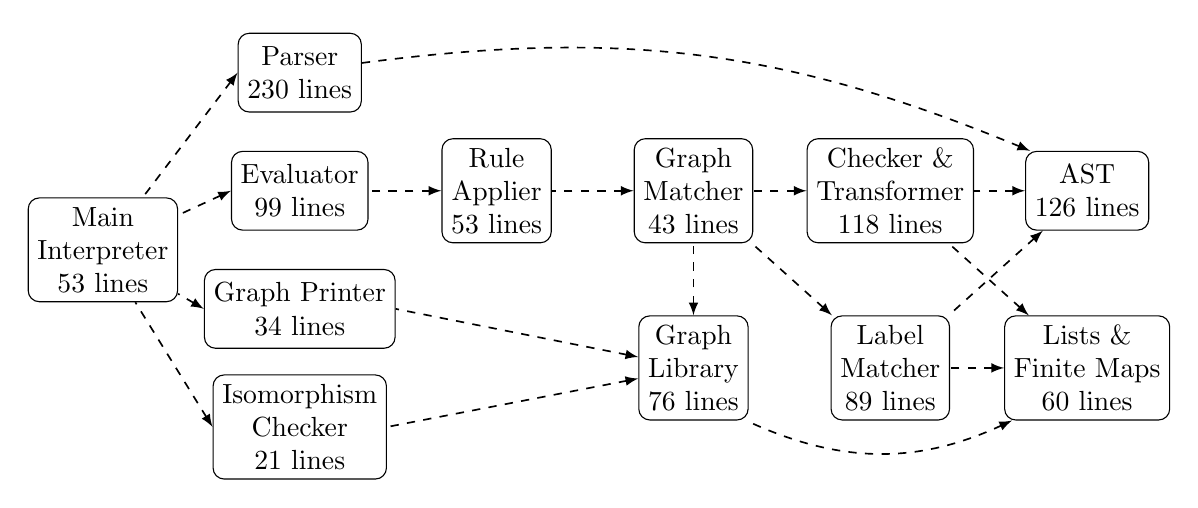
\begin{tikzpicture} [align=center]

\node(main) at (0, 0)  [box] {Main\\Interpreter\\53 lines};
\node(iso) at (2.5, -2.25) [box] {Isomorphism\\Checker\\21 lines};
\node(print) at (2.5, -0.75) [box] {Graph Printer\\34 lines};
\node(eval) at (2.5, 0.75) [box] {Evaluator\\99 lines};
\node(parser) at (2.5, 2.25) [box] {Parser\\230 lines};
\node(apply) at (5, 0.75) [box] {Rule\\Applier\\53 lines};
\node(gmatch) at (7.5, 0.75) [box] {Graph\\Matcher\\43 lines};
\node(graph) at (7.5, -1.5) [box] {Graph\\Library\\76 lines};
\node(lmatch) at (10, -1.5) [box] {Label\\Matcher\\89 lines};
\node(trans) at (10, 0.75) [box] {Checker \&\\Transformer\\118 lines};
\node(libs) at (12.5, -1.5) [box] {Lists \&\\Finite Maps\\60 lines};
\node(ast) at (12.5, 0.75) [box] {AST\\126 lines};

\draw (ast) edge[arrowin, dashed] (trans);
\draw (ast) edge[arrowin, dashed] (lmatch);
\draw (ast.145) edge[arrowin, dashed, bend right=15] (parser);
\draw (libs) edge[arrowin, dashed] (trans);
\draw (libs) edge[arrowin, dashed] (lmatch);
\draw (libs.215) edge[arrowin, dashed, bend left=25] (graph.315);
\draw (trans) edge[arrowin, dashed] (gmatch);
\draw (graph) edge[arrowin, dashed] (gmatch);
\draw (graph) edge[arrowin, dashed] (iso.0);
\draw (graph) edge[arrowin, dashed] (print.0);
\draw (lmatch) edge[arrowin, dashed] (gmatch);
\draw (gmatch.180) edge[arrowin, dashed] (apply);
\draw (apply) edge[arrowin, dashed] (eval.0);
\draw (parser.180) edge[arrowin, dashed] (main);
\draw (iso.180) edge[arrowin, dashed] (main);
\draw (eval.180) edge[arrowin, dashed] (main);
\draw (print.180) edge[arrowin, dashed] (main);

\end{tikzpicture}


}

\begin{itemize}
\itemsep1pt\parskip0pt\parsep0pt
\item
  Approx. 1000 SLOC
\item
  Exploits distinctive features of Haskell to achieve conciseness:

  \begin{itemize}
  \itemsep1pt\parskip0pt\parsep0pt
  \item
    list-comprehensions
  \item
    lazy evaluation
  \end{itemize}
\end{itemize}

\end{frame}

\begin{frame}{Performance (all result mode)}

\scalebox{0.65}{
\begin{tabular}{llrrrrrcrr}
\hline 
&  & \multicolumn{3}{c}{Output Graphs} & & && \multicolumn{2}{c}{Heap/kB}\\
Benchmark          & Host Graph & Total & Unique   & Failed & Apps & Time/s   & & Total  & Live \\
\hline 
Acyclicity test
 &             2x2 grid &      6 &         1 &     0 &     4 & $<0.01$ & &  2048 &   134 \\
 &             3x3 grid &  19770 &         1 &     0 &    12 &   12.00 & & 10240 &  3301 \\
 &             4x4 grid & - & - & - & - & $>5m$ & & - & - \\
 &           cyclic 100 &      0 &         0 &   100 &     0 &    0.06 & &  4096 &   784 \\
 &           cyclic 500 &      0 &         0 &   500 &     0 &    0.86 & & 14336 &  5651 \\
 &          cyclic 1000 &      0 &         0 &  1000 &     0 &    3.31 & & 26624 & 11053 \\
\hline
Shortest distances
 &             2x2 grid &      6 &         1 &     0 &     4 & $<0.01$ & &  2048 &   131 \\
 &             3x3 grid &  28924 &         1 &     0 &  9-14 &   19.15 & & 167936 & 58180 \\
 &             4x4 grid & - & - & - & - & $>5m$ & & - & - \\
\hline
Sierpinski
 &                gen 2 &      6 &         1 &     0 &     7 &    0.04 & &  3072 &   242 \\
 &                gen 3 & - & - & - & - & $>5m$ & & - & - \\
\hline
Transitive closure
 &            linear 05 &    866 &         1 &     0 &     6 &    0.44 & &  6144 &  1699 \\
 &            linear 10 & - & - & - & - & $>5m$ & & - & - \\
\hline
Vertex colouring
 &             2x2 grid &    480 &         2 &     0 &   6-8 &    0.07 & &  5120 &  1598 \\
 &             3x3 grid & - & - & - & - & $>5m$ & & - & - \\
\hline

\end{tabular}
}

\end{frame}

\begin{frame}{Performance (Single result)}

\scalebox{0.5}{
\begin{tabular}{llrrcrr}
\hline 
&  & & & & \multicolumn{2}{c}{Heap/kB}\\
Benchmark          & Host Graph & Apps & Time/s   & & Allocd & Live \\
\hline 
Acyclicity test
 &             3x3 grid &    12 &    0.02 & &  2048 &   129 \\
 &             5x5 grid &    40 &    0.03 & &  3072 &   382 \\
 &             7x7 grid &    84 &    0.17 & &  4096 &  1119 \\
 &             9x9 grid &   144 &    0.70 & &  6144 &  2100 \\
 &           cyclic 100 &     0 &    0.04 & &  3072 &   778 \\
 &           cyclic 500 &     0 &    0.46 & & 14336 &  5646 \\
 &          cyclic 1000 &     0 &    1.76 & & 25600 & 10368 \\
\hline
Shortest distances
 &             5x5 grid &    38 & $<0.01$ & &  3072 &   414 \\
 &             7x7 grid &    90 &    0.08 & &  4096 &  1177 \\
 &             9x9 grid &   175 &    0.39 & &  8192 &  3172 \\
\hline
Sierpinski
 &                gen 2 &     7 & $<0.01$ & &  2048 &   133 \\
 &                gen 3 &    17 &    0.14 & &  5120 &  1056 \\
 &                gen 4 &    45 &    6.52 & & 58368 & 18313 \\
 &                gen 5 & - & $>5m$ & & - & - \\
\hline
Transitive closure
 &            linear 05 &     6 & $<0.01$ & &  2048 &   144 \\
 &            linear 10 &    36 &    0.04 & &  2048 &   144 \\
 &            linear 20 &   171 &    1.67 & & 21504 &  7073 \\
 &            linear 30 &   406 &   14.39 & & 103424 & 33152 \\
 &            linear 40 &   741 &   66.31 & & 324608 & 103275 \\
 &            linear 50 & - & $>5m$ & & - & - \\
\hline
Vertex colouring
 &             3x3 grid &    27 &    0.02 & &  2048 &   140 \\
 &             5x5 grid &   125 &    0.03 & &  3072 &   999 \\
 &             7x7 grid &   343 &    0.17 & &  9216 &  3681 \\
 &             9x9 grid &   729 &    0.89 & & 25600 & 11438 \\
\hline

\end{tabular}
}

\end{frame}

\begin{frame}{Conclusions \& Further work}

\begin{itemize}
\itemsep1pt\parskip0pt\parsep0pt
\item
  We have developed a useful testing and verification tool
\item
  Gained a clear understanding of the GP 2 semantics
\item
  Become aware of `edge-cases' that might trip us up in our compiler
  work
\end{itemize}

\begin{block}{Further work}

\begin{itemize}
\itemsep1pt\parskip0pt\parsep0pt
\item
  Better error reporting
\item
  A performant compiler -- two projects underway.
\item
  Formal verification against GP 2 semantics.
\item
  GUI program editor
\end{itemize}

\end{block}

\end{frame}


\end{document}
